% ---------------------------------------------------------------------
% Content
% ---------------------------------------------------------------------

\begin{frame}[plain]
  \titlepage
\end{frame}

\begin{frame}{Outline}
\tableofcontents
\end{frame}

% ---------------------------------------------------------------------
\section{Section}
% ---------------------------------------------------------------------


\begin{frame}{Itemize and Enumerate}
    \begin{itemize}
      \item foo
      \item bar
        \begin{itemize}
          \item baz
            \begin{itemize}
              \item baz
            \end{itemize}
        \end{itemize}
    \end{itemize}
    \begin{enumerate}
      \item foo
      \item bar
        \begin{enumerate}
          \item baz
            \begin{enumerate}
              \item baz
            \end{enumerate}
        \end{enumerate}
    \end{enumerate}
\end{frame}

\subsection{Subsection}
\begin{frame}[fragile]{Code Highlighting}
  \begin{lstlisting}[language=Rust]
/// Code copied from https://doc.rust-lang.org/book/patterns.html
struct Point {
    x: i32,
    y: i32,
}

let point = Point { x: 2, y: 3 };

match point {
    Point { x, .. } => println!("x is {}", x),
}
  \end{lstlisting}
\end{frame}


\begin{frame}{Boxes and highlights}
This is \alert{highlighted}.
\begin{block}{Block}
Sample text in blue box
\end{block}
\begin{alertblock}{Alert Block}
Sample text in red box
\end{alertblock}
\begin{examples}
``Examples'' is fixed as block title.
\end{examples}
\end{frame}

\begin{frame}[fragile]{Verbatim}
\begin{lstlisting}[style=nonumbers]
Use lstlisting instead of verbatim
x
 x
  x
   x
to remove line numbers use `nonumbers` style
\end{lstlisting}
\end{frame}

\begin{frame}{Commands}
  You can use \code{\textbackslash code} to highlight stuff in monospace, e.g.
  console output or when referring to parts of code.
\end{frame}

\part{} % no section title in footer for this slides
\begin{frame}{End}
  \begin{center}
    The obligatory cat picture.\\
    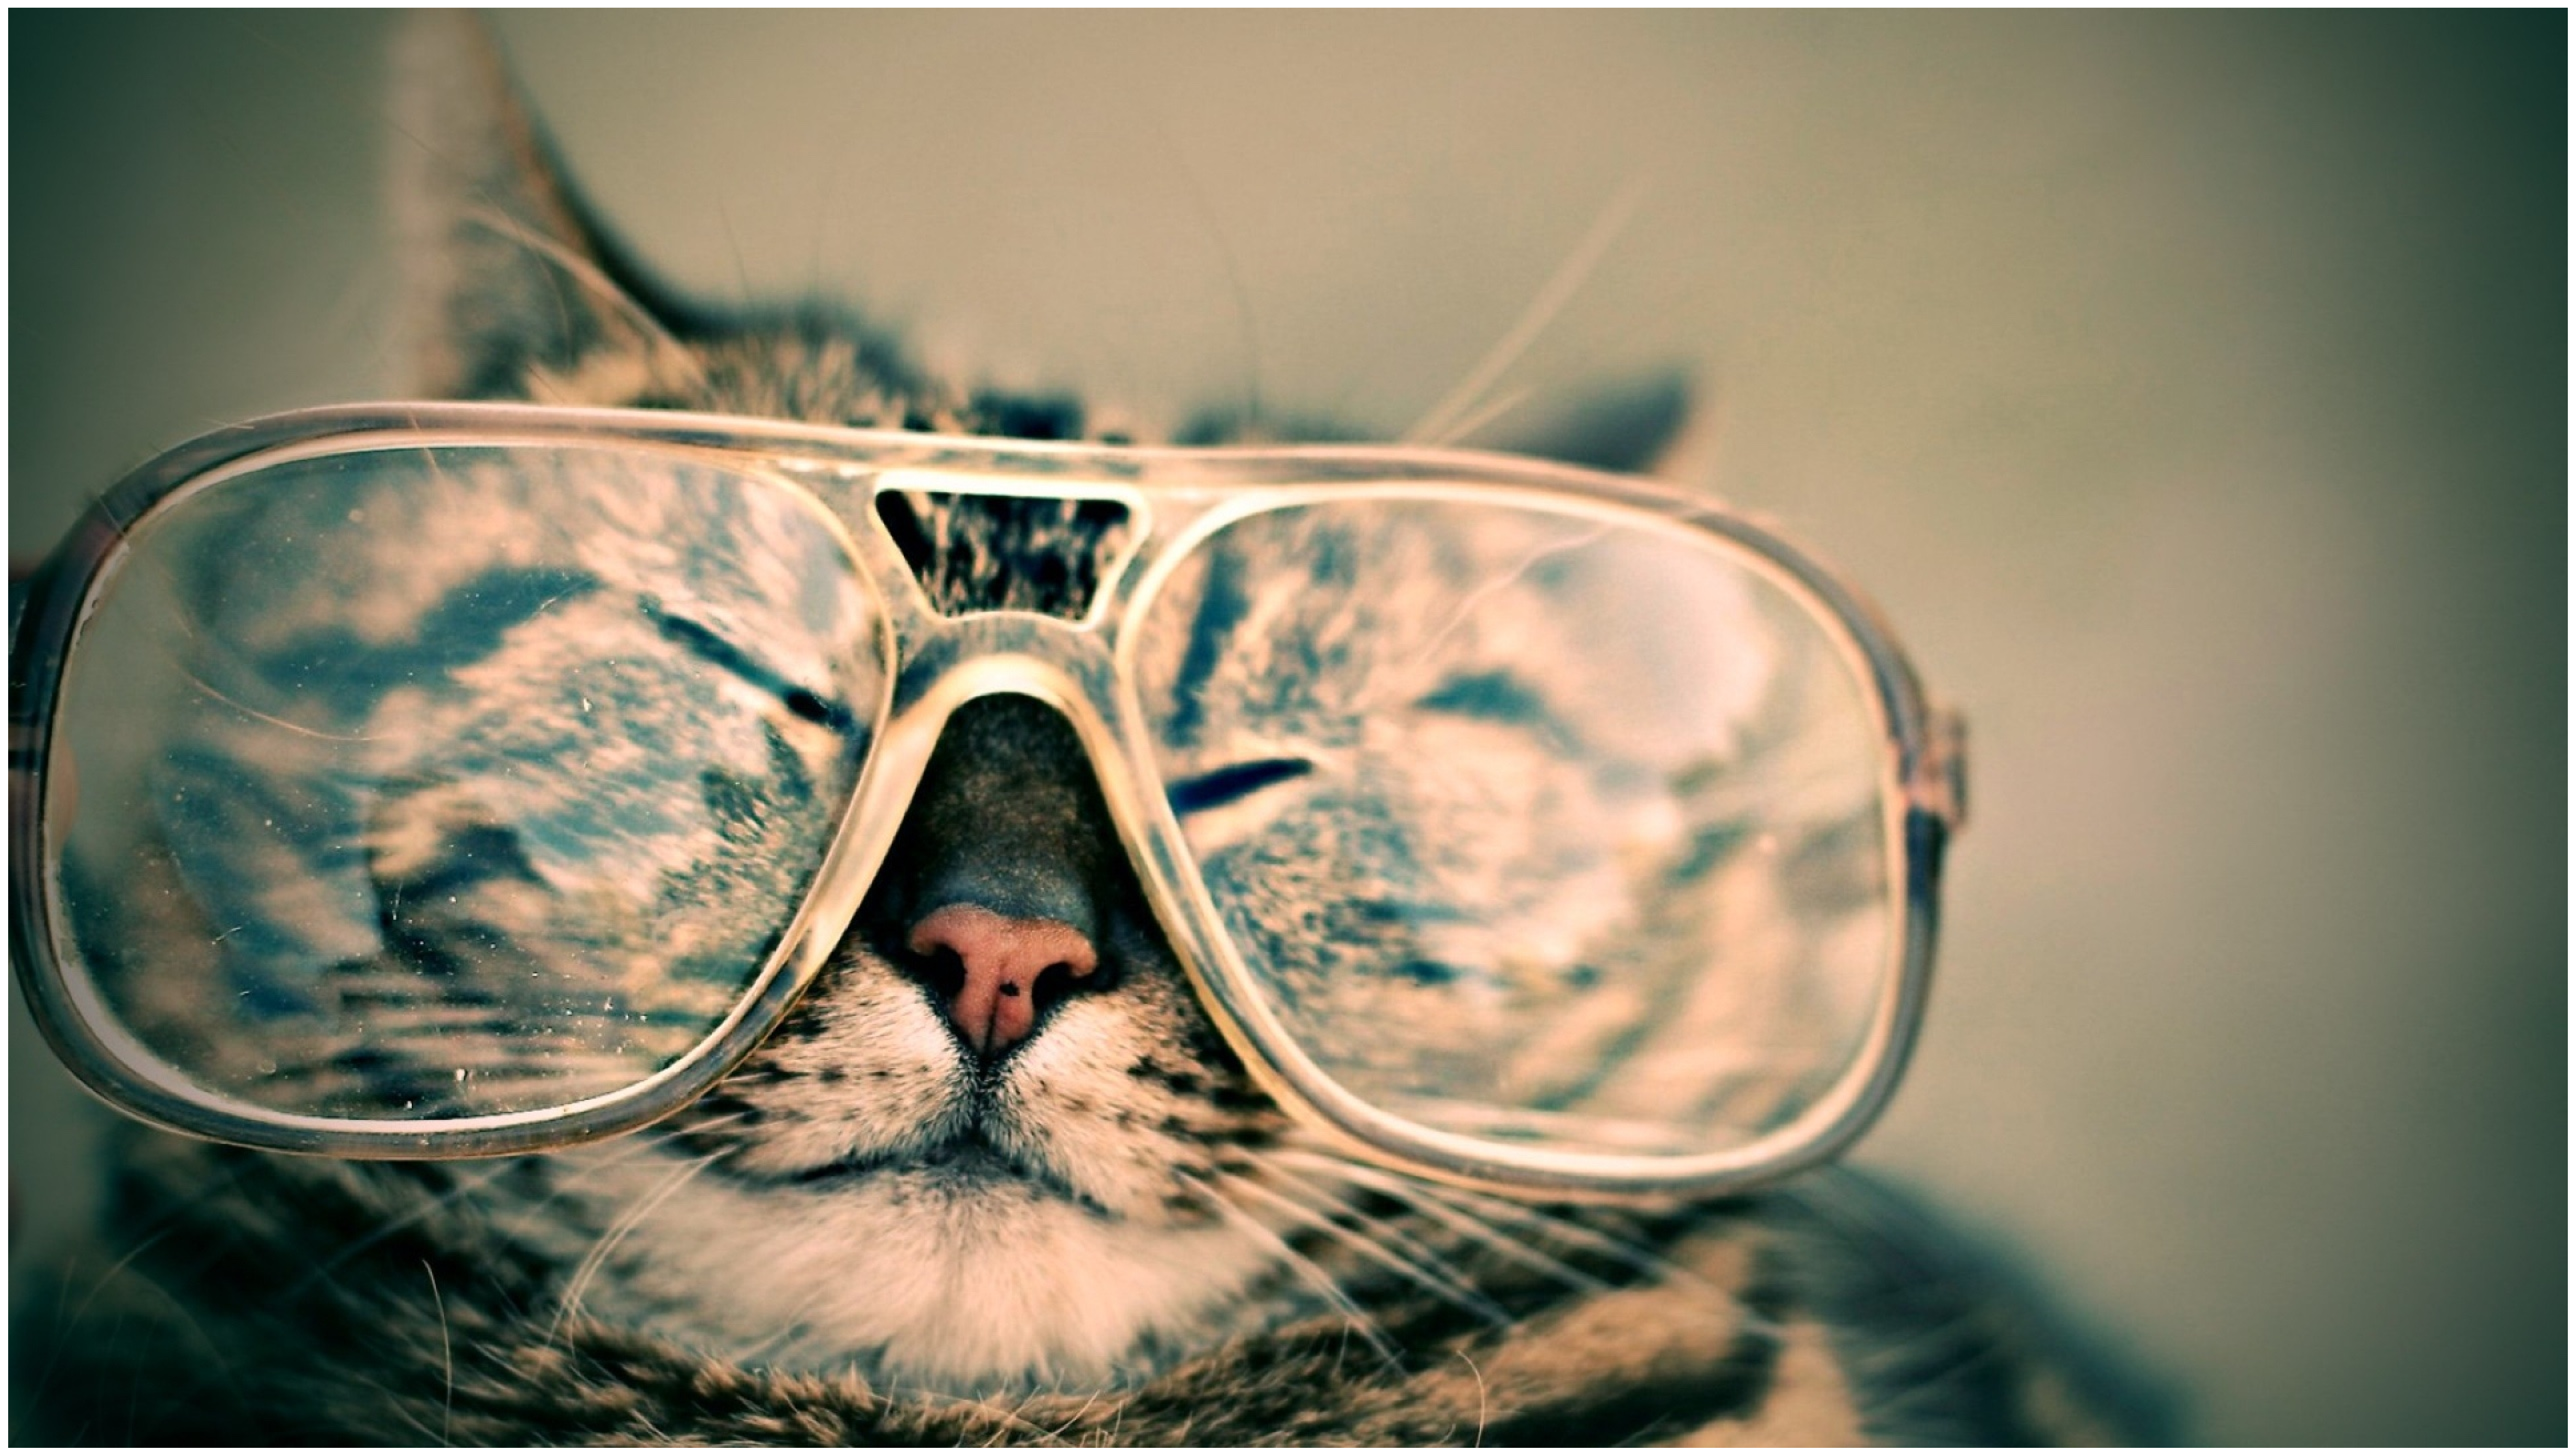
\includegraphics[height=.7\textheight]{images/octavio-fossatti-37556.eps}
    \footnote[frame]{source:
    \href{https://unsplash.com/photos/B5tUnCpJw6s}
    {https://unsplash.com/photos/B5tUnCpJw6s}}
  \end{center}
\end{frame}

%-----------------------------------------------------------------------
% Appendix
% ---------------------------------------------------------------------

\appendix
